Though the line-integrated metastable densities are one of only a few
measurements made in the development of the \acs{rpnd}, they only provide a
limited view of what is happening. In addition to the metastables are ions,
electrons, a vast array of other excited states, and the electric fields. In an
effort to expand on the details of what is occurring within the \acs{rpnd}, it
is desirable to develop a model which can infer other properties from the
metastable measurements. This is possible, because the electrons which gain
energy from the electric fields are those which excite the metastables, other
excited states, and ions. The ideal model would solve the Boltzmann equation
(equation~\ref{eq:boltzmann}) for each species, over the entire geometry, in all
dimensions, for as long as was required to reach equilibrium.

Unfortunately, these requirements are somewhat problematic. Scale lengths of 10
$\mu$m are required in order to resolve the sheath effects, resulting in
approximately $2\times10^{13}$ spatial cells. Conservatively, the time steps
would be about 1 ns in length. At a minimum, the system required about five
minutes to reach equilibrium, thus necessitating $3\times10^{11}$ solution
steps. The largest velocity can be estimated as an electron accelerated across
the full applied potential (6.6 keV), and the lowest velocity would be room
temperature (0.04 eV). This produces a velocity discretization of about
$6\times10^7$ cells. Thus the size of the parameter space in question is about
$3.6\times10^{32}$. Given that the fastest computer in the world operates at 39
petaflops, a calculation of this magnitude would take around 0.3 billion years.
Of course, this is for only a single particle species, the total number in the
system is runs in the dozens (not including the impurities).

\section{Model Development}

It should be apparent that the Boltzmann equation must be simplified in order to
model the system in a reasonable amount of time. As discussed in
chapter~\ref{chp:theory}, the most common approach to this is the use of moments
of the Boltzmann equation which drastically simplifies the velocity terms.
Frequently, the moments of the Boltzmann equation are used to develop various
fluid approximations for plasmas \cite{Chen1984} (e.g.\ the two fluid equations,
the magnetohydrodynamic equations, etc.). This approach has been tremendously
successful in the description of everything from plasma display panels
\cite{Rauf1999b} to interstellar plasmas \cite{Linde1998}.

There are some limitation to the capabilities of these fluid descriptions. For
one, they require some assumption on the form of the \acs{eedf}. Often, the
distribution is assumed to be a Maxwell-Boltzmann or Druyvesteyn, depending on
the plasma conditions. In others, an approximate solution of the Boltzmann
equation may be used to tabulate rate coefficients as a function of the mean
energy \cite{Hagelaar2005}. In addition to this issue of the \acs{eedf}, fluid
models in large or complex geometries can still be quite computationally
expensive. This can limit the number of species and reactions which can be
addressed \cite{Lieberman2005}.

In order to obtain an estimate of the detailed dynamics which occur as the
\acs{rpnd} develops, it is necessary to consider additional simplifications of
the Boltzmann equation. One such possibility is the use of a global model where
the spatial dependence of the plasma parameters is assumed. This allows global
model simulations to ignore the geometry of the system and focus on the particle
interactions for long periods of time with reasonable computational
requirements.

Here, a global model will be developed to describe the evolution of the plasma
parameters along the measurement chords during the first pulse, and before the
reflection. As was seen in the metastable measurements, there was little axial
variation over the length of the discharge. Thus, as far as the model is
concerned, variations across the beam radius are negligible. However, it has
been noted that a similar \acs{fiw} \cite{Vasilyak1994} and the same \acs{rpnd}
\cite{Weatherford2012} exhibit radial variations in emission intensity, electron
density, and metastable density. Furthermore, these variations appear to depend
strongly on the operating pressure. Unfortunately, the cause of this is not
clearly understood, though it has been suggested that high-energy electrons from
the walls may be responsible \cite{Weatherford2012a}. Lacking any empirical,
theoretical, or numerical results that provide the evolution of the radial
profile during the discharge, it is necessary to assume one. In this case, the
plasma will be assumed to be uniform across the diameter of the discharge. This
assumption will affect the accuracy of the inferred plasma parameters, however
future improvements in the understanding of these radial variations can be
easily incorporated into the described model.

\subsection{Continuity Equation}

The global model begins with equation~\ref{eq:cont}, the continuity equation.
Having assumed that the spatial variations are zero, the equation reduces to,
\begin{equation}
  \frac{d n_\alpha}{dt} = G_\alpha - L_\alpha,
  \label{eq:zdmcont}
\end{equation}
where $\alpha$ identifies the particle species, $G$ is the gain term, and $L$ is
the loss term. The gain and loss terms represent a large range of possible
processes which are determined, in part, by the species under consideration. In
this model, only helium, excited helium states, helium ions, and electrons will
be treated. While impurities and dimers are very much a part of the discharge,
this occurs on time scales that are relatively long in comparison to the
excitation period. As was noted in chapter~\ref{chp:metastables}, only 140 ns
elapse before the reflection arrives at the plasma, while the e-folding time of
the fastest decay is about 25 $\mu$s.

Given the species of the system, there are several processes that should be
given consideration for inclusion in the model.
\begin{enumerate}
  \item Electron impact ionization 
  \item Electron impact (de)excitation 
  \item Atomic impact (de)excitation
  \item Atomic excitation transfer
  \item Dielectronic recombination
  \item Three-body recombination
  \item Radiative decay
  \item Diffusion
\end{enumerate}
As with the impurities and dimer formation, diffusion occurs on a much longer
time scale, and thus is neglected. Three-body recombination in the volume of the
discharge is not important at the estimated temperatures and densities
\cite{Lieberman2005}, therefore this too is neglected. Dielectronic
recombination is also quite rare, however the process was incorporated as part
of the early models and thus maintained through the final revision. Inter-atomic
excitation and de-excitation is not generally considered important given the low
energies of the atoms in a discharge. However, excitation \emph{transfer} can be
an important process in gaseous discharges \cite{Lieberman2005}, making their
inclusion necessary. Also important are the electron impact ionizations and
excitations, as well as the radiative decay of the atoms.

Given these processes, it is possible to rewrite equation~\ref{eq:zdmcont} as,
\begin{multline}
  \frac{dN_i}{dt} =   n_e \left[       \sum_{j\neq i} N_j K^e_{ji}(T_e) 
                                 - N_i \sum_{j\neq i}     K^e_{ij}(T_e) \right]
                        + \left[       \sum_{j\neq i} N_j K^o_{ji} 
                                 - N_i \sum_{j\neq i}     K^o_{ij}      \right] \\
                    + N_g \left[       \sum_{j\neq i} N_j K^a_{ji} 
                                 - N_i \sum_{j\neq i}     K^a_{ij}      \right].
  \label{eq:gcont}
\end{multline}
In these equations, the subscripts of $i$ and $j$ represent states of helium,
$N$ is a state density, $K$ is a rate coefficient, $T_e$ is the electron
temperature, and $N_g$ is the neutral helium density. The first subscript of the
rate coefficients represents is the initial excited state while the second
coefficent represents the final excited state. Therefore, $K_{ij}$ represents a
process that depopulates state $i$ in favor of state $j$.

This equation is split into three sets of processes, represented by the
superscripts of the rate coefficients: $e$ - electronic, $o$ - optical, and $a$
- atomic. The first bracketed term on the right hand side contains all the rate
coefficients for electron impact excitation and de-excitation, including
ionization processes. The second bracketed term contains the rate coefficients
for optical transitions in and out of the state. The final bracketed term
contains the gains and losses as a result of excitation transfer caused by
collisions with the ground state. Collisions between excited states are
neglected given their relatively low densities.

The rate coefficients in equation~\ref{eq:gcont} are compiled from a number of
different sources. This is particularly straight forward in the case of the
optical and atomic transitions, as neither features any dependence on the
\acs{eedf}. The optical transition rates and level energies were obtained from
the NIST Atomic Spectra Database \cite{Kramida2012}. The excitation transfer
rate coefficients were from the studies of Catherinot and Dubreuil
\cite{Catherinot1981, Dubreuil1980}. These coefficients only covered the
transitions of $\Delta n=0$ for $n=3,4$ and no constants were found for other
$n$ or $\Delta n\neq 0$.

The semi-empirical relations derived by Ralchenko et al. \cite{Ralchenko2008}
were used to calculate the electron (de)excitation and ionization cross sections
through $n=4$. These represent the most accurate set of cross sections available
for neutral helium and have a quoted accuracy of 10-30\% for $\Delta S=0$, and
$\ge30$\% for $\Delta S \neq 0$. These cross sections can be used to calculate
the rate coefficients for each reaction using equation~\ref{eq:rate}. However,
this poses the problem of what kind of energy distribution to use.

\subsection{Distribution Effects}

Per the discussion of the Boltzmann equation in chapter~\ref{chp:theory}, there
are two readily available equilibrium solutions: the Maxwell-Boltzmann
distribution, and the Druyvesteyn distribution. However, research by
Starikovskaia and Starikovskii \cite{Starikovskaia2001} has shown that the
\acs{eedf} in a nitrogen \acs{fiw} can deviate from both of these solutions.
Such a result is not too surprising given the non-equilibrium nature of the
\acs{fiw} discharge. Since the \acs{rpnd} shares many of these same properties,
it is possible that the equilibrium solutions do not apply to the \acs{rpnd}
either.

In order to better understand how the energy distributions may behave in a
\acs{rpnd}, a numerical study of the \acs{eedf} in a helium \acs{rpnd} was
conducted. First, \acs{pic} code was used to simulate the effect of a voltage
pulse on electrons in a quasi zero-dimensional geometry. This provided a series
of baseline \acs{eedf}s which varied with respect to time. Then, at each time
point, the mean energy was calculated from the \acs{pic} results. The mean
energy was then used to generate equivalent approximate solutions of the
Boltzmann equation, and Maxwell-Boltzmann distributions.

\acs{pic} simulations do not attempt to solve the Boltzmann equation directly.
In essence, they are a model of an actual experiment and can have one, two, and
three dimensional geometries. They consider a population of discrete
macro-particles within the specified geometry, subject to specified fields, and
governed by the basic laws of motion \cite{Birdsall1991}. While each
macro-particle has a specific location, velocity, charge, and mass, it is not
the same as a single physical particle. It also possesses a statistical weight
which allows it to represent a \emph{group} of physical particles. Provided
enough macro-particles, their velocities can be compiled to construct an
estimate of the real \acs{eedf}.

The process by which the \acs{pic} simulation is conducted is illustrated in
figure~\ref{fig:pic}.
\begin{figure}
  \centering
  \setlength{\unitlength}{4.8in}
\begin{picture}(1.0, 0.5)
   \put(0.10, 0.35){\framebox(0.35, 0.10){\parbox{0.35\unitlength}{\footnotesize\centering Integration of equations \\ of motion, moving particles \\ $\vec{F}_i \rightarrow \vec{v}'_i \rightarrow x_i$}}}
   \put(0.45, 0.40){\line( 1,  0){0.10}}
   \put(0.55, 0.35){\framebox(0.35, 0.10){\parbox{0.35\unitlength}{\footnotesize\centering Particle loss/gain \\ at the boundaries \\ (emission, absorption, etc.)}}}
   \put(0.90, 0.40){\line( 1,  0){0.05}}
   \put(0.95, 0.40){\line( 0, -1){0.10}}
   \put(0.70, 0.20){\framebox(0.30, 0.10){\parbox{0.30\unitlength}{\footnotesize\centering Monte Carlo collisions \\ $\vec{v}'_i \rightarrow \vec{v}_i$}}}
   \put(0.95, 0.20){\line( 0, -1){0.10}}
   \put(0.95, 0.10){\line(-1,  0){0.10}}
   \put(0.60, 0.05){\framebox(0.25, 0.10){\parbox{0.25\unitlength}{\footnotesize\centering Weighting \\ $(x,\vec{v})_i \rightarrow (\rho, \vec{J})_j$}}}
   \put(0.60, 0.10){\line(-1,  0){0.20}}
   \put(0.15, 0.05){\framebox(0.25, 0.10){\parbox{0.25\unitlength}{\footnotesize\centering Integration of field \\ equations on grid \\ $(\rho, \vec{J})_j \rightarrow (\vec{E},\vec{B})_j$}}}
   \put(0.15, 0.10){\line(-1, 0){0.10}}
   \put(0.05, 0.10){\line( 0, 1){0.10}}
   \put(0.00, 0.20){\framebox(0.20, 0.10){\parbox{0.20\unitlength}{\footnotesize\centering Weighting \\ $(\vec{E},\vec{B})_j \rightarrow \vec{F}_i$}}}
   \put(0.05, 0.30){\line( 0,  1){0.10}}
   \put(0.05, 0.40){\line( 1,  0){0.05}}
   \put(0.46, 0.22){\Huge $\circlearrowright$}
   \put(0.4725, 0.2275){\footnotesize\centering $\Delta t$}
\end{picture}

  \caption{Schematic description of the \acs{pic} simulation process, adapted
    from \cite{Birdsall1991}.}
  \label{fig:pic}
\end{figure}
The process begins with the definition of a system geometry and an applied
electromagnetic field, $\vec{E}$ and $\vec{B}$. In this case, the system is
strictly one-dimensional, so each macro-particle only possess one spatial
component, $x$. However, to account for magnetic field effects, each
macro-particles possesses three velocity components, $\vec{v}$. This is followed
by an initialization of the particle positions and velocities. The number of
particles and the their positions are usually chosen to given a specific plasma
density, and the velocities are often chosen to represent some initial
distribution of energy. The Lorentz equation, $\vec{F} = q(\vec{E} +
\vec{v}\times\vec{B})$, is then used to push each particle to a new position for
a given time step, $\Delta t$. Particles born or lost at the boundaries are then
accounted for. This is followed by a modeling of collisions (including
ionization and excitation) using Monte Carlo techniques \cite{Birdsall1991}. The
charges of the macro-particles are then weighted to a spatial grid, and the
fields are recalculated, and the next time step begins.

The XPDP1 code, developed by Verboncoeur et al. \cite{Verboncoeur1993}, was used
to conduct the \acs{pic} simulations. The code was originally designed to
simulate a one-dimensional discharge between two parallel electrodes. However,
the electrodes complicate the study of the \acs{eedf}. Charged particle
collection near the boundaries will introduce spatial variations in the
\acs{eedf}. In addition, such collection can lead to large regions of space
charge which can shield out the applied electric field. In order to address
these issues, the code was modified to use periodic boundary conditions. Such
conditions result in a quasi zero-dimensional simulation, equivalent to a plasma
of infinite extent. This eliminates the issue of spatial variations in the
\acs{eedf}.

Previous measurements of the electric field in a similar \acs{fiw} suggested
that the electric field values varied from 0-350 Td \cite{Takashima2011}. Based
on this, it was decided to examine the distribution characteristics from 10-600
Td. This range should be adequate to cover all conditions within the \acs{rpnd}
in question. The background gas was helium at a pressure of 2.0 Torr. The
initial plasma was assumed to be quasineutral with a density of
$1.0\times10^{8}$ cm$^{-3}$ and 10$^4$ macro-particles. Electrons were
initialized with a thermal energy of 2.0 eV, and the helium ions were given an
initial energy of 0.025 eV. 

The internal set of cross sections, which include elastic scattering,
excitation, and charge exchange were used. The cross sections have a
semi-empirical form which increases linearly with energy to a peak value after
which it declines as the logarithm of the energy, divided by the energy. The
time domain of the simulation was 10 ns, approximately the time required for the
\acs{eedf} to reach equilibrium with the applied field. The distributions from
the \acs{pic} simulations were sampled every 0.25 ns. The spatial domain was
discretized at 1 $\mu$m intervals over a total domain of 10 cm. Based on the
highest energy electrons in the system, a time step of $4\times10^{-13}$ s was
chosen in order to satisfy the Courant-Friedrich-Lewy stability condition.

BOLSIG+ was used to obtain the approximate solutions of the Boltzmann equation
\cite{Hagelaar2005}. This is a publicly available computer code which uses the
two-term expansion of the Boltzmann equation to solve for the \acs{eedf} for a
given electric field. In this approach, Legendre polynomials are used to expand
the \acs{eedf} into an equilibrium solution and a relatively small
non-equilibrium component. This implied assumption, that the distribution is
accurately represented by a small perturbation superimposed on an equilibrium
solution, puts constraints on the magnitude of the reduced electric field. In
the case of BOLSIG+, the solver fails to converge for fields approaching 1000
Td.

The solver was inititialized with the cross sections for helium generated by
Alves and Ferreira \cite{Alves2013}. The temporal growth model for electrons was
used, and the electron-electron collisions were not neglected as a result of the
low ionization fraction in the \acs{rpnd}. Solutions were calculated for a range
of electric fields and then tabulated according to their mean energy. A nearest
neighbor interpolation scheme was used to generate an \acs{eedf} for the mean
energies from the \acs{pic} simulations.

These same energies were used to determine equivalent Maxwell-Boltzmann
distributions for comparison. The results of these calculations can be seen in
figure~\ref{fig:picmb},
\begin{figure}
  \centering
  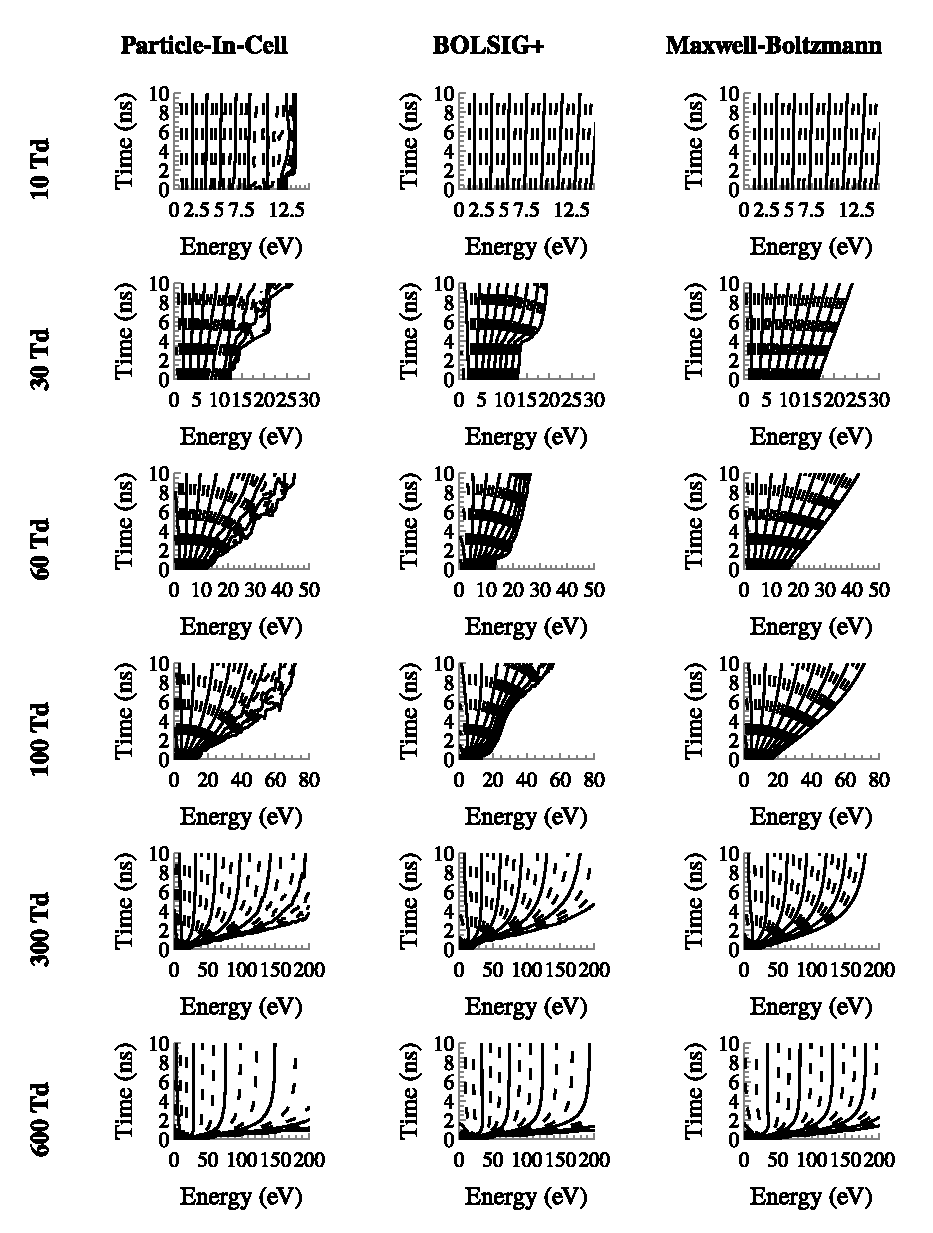
\includegraphics{./chapters/modeling/figures/picmb.eps}
  \caption{Contour plots of the \acs{eedf}s determined from \acs{pic}
    simulations, and the corresponding Maxwell-Boltmzann distributions for a range
    of electric fields.}
  \label{fig:picmb}
\end{figure}
as a series of contour plots comparing the results for each approach. The
jaggedness of the \acs{pic} simulations results from the finite number of
particles in the system and the low probability of high energy electrons. This
problem is ameliorated at higher electric fields where the probability of
high-energy electrons increases. An increase in the number of electron
macro-particles, resulting from ionization, also helps to reduce this effect.

At 10 Td, the \acs{eedf}s are relatively unchanged over the duration of the
simulation. The subtle slopes of the contours suggest a small increase in the
overall temperature and energy of the system. The rate of increase in
temperature increases as the value of the electric field is increased. At 30 Td,
the contours of each approach are essentially linear with similar slopes. The
only noticeable deviation is the closer spacing of the contours from BOLSIG+.
Thus the probability distribution falls off faster with energy for this case
relative to the \acs{pic} simulations and the corresponding Maxwell-Boltzmann
distributions.

At 60 and 100 Td, the \acs{pic} results and Maxwell-Boltzmann distributions
continue to feature contour spacings which increase linearly with time. In
contrast, the BOLSIG+ solutions have contour spacings which are monotonically
increasing, but at a rate which varies in time. Additionally, the spacing
between the various levels is less consistent than for the \acs{pic} simulations
or the Maxwell-Boltzmann distributions. By the end of the simulation period, the
overall width of BOLSIG+ contours is less than either of the other approaches.

However, by 300 and 600 Td the situation has slight changed. The
Maxwell-Boltzmann distributions show consistently less breadth than the
\acs{pic} results of the BOLSIG+ solutions. Close examination shows that the
\acs{pic} simulations have larger populations of low energy (less than 20 eV)
and high energy (greater than 100 eV) electrons. This can be traced back to the
form of the helium cross sections used in XPDP1. The only reactions available to
electrons in the simulation are elastic scattering, excitation (19.6 eV
threshold), and ionization (24.6 eV threshold). Thus the electron population is
depleted at values above around 20 eV, as a result of these inelastic processes.
Likewise, the electron population begins to rebound at higher energies as the
inelastic processes turn off. The Maxwell-Boltzmann solutions are quite simple
and do not account for the variation of the cross sections with respect to
energy. This explains the increased consistency of the \acs{pic} and BOLSIG+
results at high electric field values.

Generally, the Maxwell-Boltzmann results appear to provide the best match to the
\acs{pic} simulations at electric fields of 100 Td and below. At higher fields,
the BOLSIG+ results provide a better approximation of the \acs{pic} results.
If the electric fields measured by Takashima et al.\ are the same as those in the
\acs{rpnd} studied here, then the Boltzmann solver would be the best choice at
the peak field values. However, for a very large fraction of the time, the
Maxwell-Boltzmann distribution would appear to provide the best approximation of
the electron distributions in the system. As a result, it was decided to use
this distribution for the development of the global model.

\subsection{Energy Equation}

Given a form for the distribution function, it is now possible to calculate the
rate coefficients in equation~\ref{eq:gcont} at each time step. However, as was
seen in figure~\ref{fig:picmb}, the distribution function changes over time. In
that case, the \acs{pic} simulations were used to calculate the mean electron
energy which, in turn, was used to determine the appropriate Maxwell-Boltzmann
distribution. However, as of yet, no mechanism has been provided to evolve the
mean electron energy in the absence of such simulations.

With suitable assumptions, equation~\ref{eq:energy} (the second moment of the
Boltzmann equation) can provide the means to evolve the mean energy with each
time step. Given the assumptions underlying the global model, the spatial
derivatives can be neglected so that
\begin{equation}
  \frac{d}{dt}\left(\frac{3}{2}p_e\right) =
  \frac{d}{dt}\left(\frac{3}{2}p_e\right)\bigg|_\mathrm{coll}.
\end{equation}
Using the isothermal equation of state, $p=n\kB T$, this can be rewritten as,
\begin{equation}
  \frac{d}{dt}\left(\frac{3}{2}n_e\kB T_e \right) =
  \frac{d}{dt}\left(\frac{3}{2}n_e\kB T_e \right)\bigg|_\mathrm{coll}.
  \label{eq:energy2}
\end{equation}
The term on the RHS is the collision operator which expresses energy gained or
lost by electrons\footnote{In some plasmas, it is desirable to also treat gas
heating with a similar equation as it can have an appreciable impact on certain
rate constants. However, as noted in chapter~\ref{chp:metastables}, the gas
temperature of the \acs{rpdn} in question remains at room temperature.} in
particle collisions.

Several different forms of particles collisions must be considered by the global
model. Once the electron population surpasses the 19.6 eV threshold, a great
deal of energy will be exchanged with excited helium species through inelastic
collisions. In addition, the electron population will tend to thermalize with
the background gas over long periods of time via elastic collisions. Finally,
energy is gained by the electrons through the applied electric field. Together,
these phenomena replace the term on the RHS of equation~\ref{eq:energy2} with,
\begin{equation}
  \frac{e^2n_eE(t)^2}{m_ek_m(T_e)N_g}
  - n_ek_m(T_e)N_g\left(\frac{3m_e}{M}\right)\frac{3}{2}\kB(T_e-T_g)
  - n_e \sum_i \sum_{j\neq i} K^e_{ij}N_i\Delta\epsilon_{ij},
  \label{eq:energyparts}
\end{equation}
where $E(t)$ is the time-varying electric field, $k_m$ is the electron momentum
transfer frequency, and $\Delta\epsilon_{ij}$ is the energy lost or gained by
the electron in atomic (de)excitation reactions. The first term includes the DC
conductivity \cite{Lieberman2005} of the plasma, and accounts for the heating of
the electrons by the electric field. The second term is the elastic cooling of
the electrons by the neutral atoms, where the gas temperature is assumed fixed.
The third term is the energy gained or lost by the electrons in atomic
(de)excitation reactions. Equation~\ref{eq:energyparts}, with
equations~\ref{eq:energy2} and~\ref{eq:gcont} are sufficient to solve for the
evolution of the electron temperatures, electron densities, excited state
densities, and plasma emissions as functions of time.

\subsection{Model Solutions}


\section{Plasma Parameters}



\section{Summary}



